\documentclass{article}
\usepackage[dblblindworkshop]{neurips_2026}
\workshoptitle{Preprint}
\usepackage[utf8]{inputenc}
\usepackage[T1]{fontenc}
\usepackage{hyperref,url,booktabs,amsfonts,amsmath,microtype,xcolor,graphicx}
\hypersetup{pdfauthor={Rami Alobaidy},pdftitle={AutoPareto: Auditing Fixed-Time Autonomous Transformer Search with Matched-Exposure Verification},colorlinks=true,citecolor=blue,linkcolor=blue,urlcolor=blue}
\newcommand{\APParams}{29.36}
\newcommand{\APBPB}{1.141837}
\newcommand{\APSpeed}{383.02}
\newcommand{\APTime}{385.02}
\newcommand{\APWall}{508.23}
\newcommand{\APMemory}{162.88}
\newcommand{\ARParams}{50.33}
\newcommand{\ARBPB}{1.099803}
\newcommand{\ARSpeed}{192.93}
\newcommand{\ARTime}{696.16}
\newcommand{\ARWall}{813.45}
\newcommand{\ARMemory}{250.88}
\newcommand{\DecodeRatio}{1.99}
\newcommand{\MemoryReduction}{35.1}
\newcommand{\ParameterReduction}{41.7}
\newcommand{\BPBCost}{0.042034}
\newcommand{\PanelN}{21}
\newcommand{\BudgetN}{8}
\newcommand{\TimeN}{4}
\newcommand{\TokenN}{4}
\newcommand{\TimeBest}{1.103402}
\newcommand{\TokenBest}{1.124312}
\newcommand{\BudgetParetoN}{0}
\newcommand{\BLiMPLower}{51}
\newcommand{\BLiMPTied}{1}
\newcommand{\BLiMPHigher}{15}
\newcommand{\APKV}{1.992}
\newcommand{\ARKV}{3.984}
\newcommand{\KVReduction}{50}
\newcommand{\BLiMPHeldoutCorr}{-0.969}
\newcommand{\BLiMPDepthCorr}{0.717}
\newcommand{\BLiMPParamCorr}{0.680}
\newcommand{\BatchOnlyBPB}{1.1040}
\newcommand{\BatchOnlyTokens}{88.1}
\newcommand{\NonBatchOnlyBPB}{1.2188}
\newcommand{\NonBatchOnlyTokens}{94.4}

\title{AutoPareto: Auditing Fixed-Time Autonomous Transformer Search\\with Matched-Exposure Verification}
\author{Rami Alobaidy}
\begin{document}
\maketitle

\begin{abstract}
When an autonomous researcher optimizes models under a wall-clock budget, the budget becomes part of the objective: a program that trains faster is handed more data before anyone scores it. We make this concrete in AutoPareto, an autonomous Transformer researcher that edits its own training source under measured quality, cached-decode throughput, and inference-memory objectives, and that preserves every hypothesis, patch, and parent link it produced. Under a 300-second training contract, the candidates it compared consumed between 88.9M and 251.8M training tokens, and the recipe that won on validation quality had seen 1.8 times the data of the strongest quality-only baseline. Freezing seven archived recipes and retraining them on unseen seeds at an identical 201.3M-token budget reorders them: the agent's selected recipe loses its discovery-stage quality lead, while the deployment trade-off it found survives intact at 1.99 times the cached-decode throughput, 41.7\% fewer parameters, and 35.1\% less allocated inference memory. A registered prospective comparison of fixed-time against fixed-token contracts is reported as an exploratory prefix. Enforcing the contract took three human repairs, including one in which eleven untimed warm-up updates were quietly donating 5.77M tokens of free training to every candidate. We preserve the complete record behind each claim: every agent hypothesis and source patch, parent lineage, training and confirmation seeds, recipe and checkpoint hashes, registered contracts, and the raw per-repetition inference measurements, and we release the frozen recipe sources, protocol manifests, and per-seed results, so every number here can be re-derived without retraining. Resource contracts belong in the experimental specification of autonomous ML research, not only in its reporting.
\end{abstract}

\section{Introduction}
Autonomous research agents are now evaluated by giving them a task, a machine, and a budget, then reading off whichever candidate scores best. The budget is usually wall-clock time, because time is what a GPU actually rations. That choice has a consequence that is easy to miss: when the agent may edit the training program itself, an edit that raises training throughput does not merely make the experiment cheaper, it buys the candidate more optimizer updates and more tokens before the score is taken. The agent is then rewarded for two different things at once, and the reward signal does not distinguish them.

This paper measures how large that effect can be, in a setting where the entire research trajectory was retained. \textbf{AutoPareto} is an autonomous Transformer researcher built on the fixed-time, single-file training loop of the autoresearch project \citep{autoresearch}. It receives a parent training program and the results of its own prior attempts, proposes a hypothesis, edits \texttt{train.py}, and is scored by protected evaluators on validation bits per byte, cached-decode throughput, and peak allocated inference memory. Nothing about the evaluators is reachable from the editable surface. Across three 25-attempt campaigns the agent produced a lineage of architecture, optimizer, batching, and schedule edits, and its highest-scoring recipe reached a validation BPB of 1.0933 against 1.0950 for the strongest quality-only comparator.

Those two numbers were produced under very different amounts of training. Under the 300-second contract, the seven recipes we later verified had consumed between 88.9M and 251.8M tokens, a factor of 2.8, and the winning recipe had processed 1.80 times as many tokens as the recipe it beat. The discovery-stage comparison is therefore not a comparison of programs at equal exposure, and its 0.0017 BPB margin is small relative to that difference.

We resolve this the only way the archive allows: we froze seven recipes as exact source files, retrained each on three seeds that had never been used, and gave every one of them exactly 201,326,592 counted tokens. Under that protocol the ranking changes. The agent's selected recipe, AP292, falls behind the quality-only comparator on held-out BPB, reversing the discovery-stage ordering, while its efficiency advantages persist at identical tokens, updates, and batch size. The autonomous search found something real. It was a deployment result, not the quality result its own contract appeared to certify.

Getting to a contract that could be enforced at all took work that we report rather than hide. Three human repairs stand between the original loop and the numbers in this paper, and one of them, the discovery that eleven untimed warm-up updates were donating 5.77M tokens of unbudgeted training to every candidate, is the same class of error the paper is about: a resource leak that no score would have revealed.

\paragraph{Contributions.}
\begin{enumerate}\setlength{\itemsep}{1pt}
\item We characterize the resource contract as an experimental variable in autonomous ML research and quantify its reach in a real campaign: under a fixed-time contract, the candidates being ranked differed by a factor of 2.8 in training exposure, and the apparent winner was among the most heavily trained.
\item We introduce matched-exposure verification for autonomous discoveries and apply it to seven frozen recipes on unseen seeds. It removes the discovery-stage quality advantage of the selected recipe and preserves a substantial, independently measured deployment trade-off.
\item We provide an auditable autonomous research record, covering agent hypotheses, source patches, parent lineage, failures, registered contracts, seeds, source and checkpoint hashes, and raw per-repetition measurements, together with the contract-enforcement and inference-correctness repairs that the measurements depend on and a registered prospective design for testing whether the contract itself redirects the agent's search.
\end{enumerate}

\section{The AutoPareto research system}\label{sec:system}
\paragraph{Agent and editable surface.} The research agent is Codex CLI 0.153.0 running \texttt{gpt-5.6-sol} at high reasoning with a 600-second per-call timeout, invoked headlessly in a fresh ephemeral container for each attempt. It receives five staged files and may write exactly one of them, \texttt{train.py}. The dataset, the tokenizer, the controller, and the evaluators lie outside that surface and are hashed on every attempt, so a candidate cannot alter how it will be measured. Campaign histories are per-arm and are never crossed, and the agent sees no downstream benchmark, no prior paper draft, and no results from any other arm.

\paragraph{Objective contract.} Three quantities are returned after each attempt. Validation bits per byte is the quality signal; expressing cross-entropy per byte of the original UTF-8 stream keeps candidates comparable when their tokenization cost per sequence differs. Cached-decode throughput is the serving mode that architectural depth and KV-cache changes actually affect, measured on a fixed protected prompt in BF16 at batch one with 256 input and 256 generated tokens, of which the 255 single-token cached steps after prefill are timed. Peak allocated inference memory bounds deployability on a fixed device. Appendix~\ref{app:measure} gives the exact measurement boundaries.

\begin{figure}[t]
\centering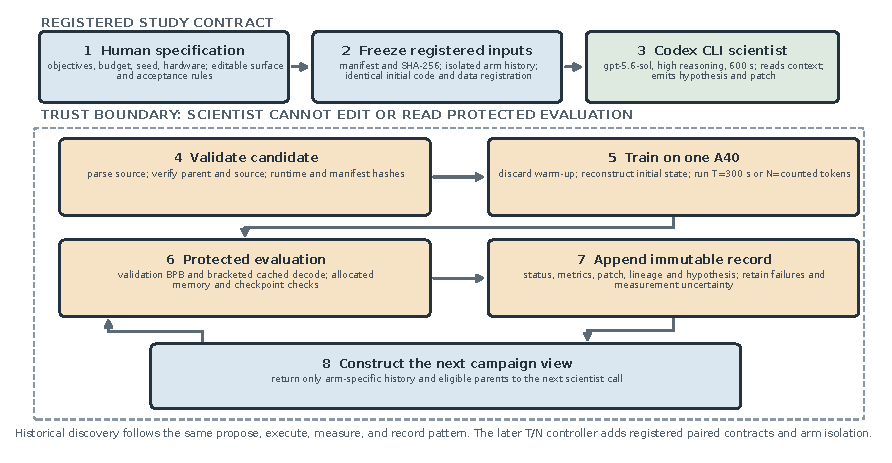
\includegraphics[width=\linewidth]{figures/research_loop.pdf}
\caption{The executed research loop and its trust boundary. Humans register the scientific contract; the controller freezes and hashes the inputs; the agent emits a hypothesis and a source patch; protected code validates, trains, measures, and appends an immutable record. The agent can neither read nor modify the protected evaluators, and only an arm-specific campaign view is returned to the next call.}\label{fig:loop}
\end{figure}

\paragraph{Research loop.} Each iteration begins from the human-defined contract. The agent receives the current campaign context, records a hypothesis and an intended change, and proposes a patch. The controller validates the patch against the declared parent and source hashes, runs training on the A40 worker, checks the resulting checkpoint, calls the protected quality and deployment evaluators, and appends an immutable record before constructing the next arm-specific context. Figure~\ref{fig:loop} shows the loop and the trust boundary. Parents are chosen within an arm from recorded lineage; under the executed manifest a candidate whose quality is valid remains eligible as a parent even when its speed measurement is uncertain, though such candidates are not eligible for the frontier. Attempts that fail technically, complete with poor quality, or complete with uncertain timing are preserved as distinct states rather than dropped.

\section{Autonomous search under a fixed-time contract}\label{sec:search}
\paragraph{Task and contract.} The registered baseline is an eight-layer, 512-wide decoder-only Transformer with 50,332,176 parameters trained on ClimbMix-400B-shuffle with a project-specific 8,192-entry vocabulary and 2,048-token packed sequences, on one NVIDIA A40. Each attempt receives a protected training budget of 300.000 measured seconds and stops after the first completed optimizer update at or beyond that boundary. The allowance is an immutable protected constant, chosen so that a 25-attempt campaign fits inside a single-GPU session.

\begin{figure}[t]
\centering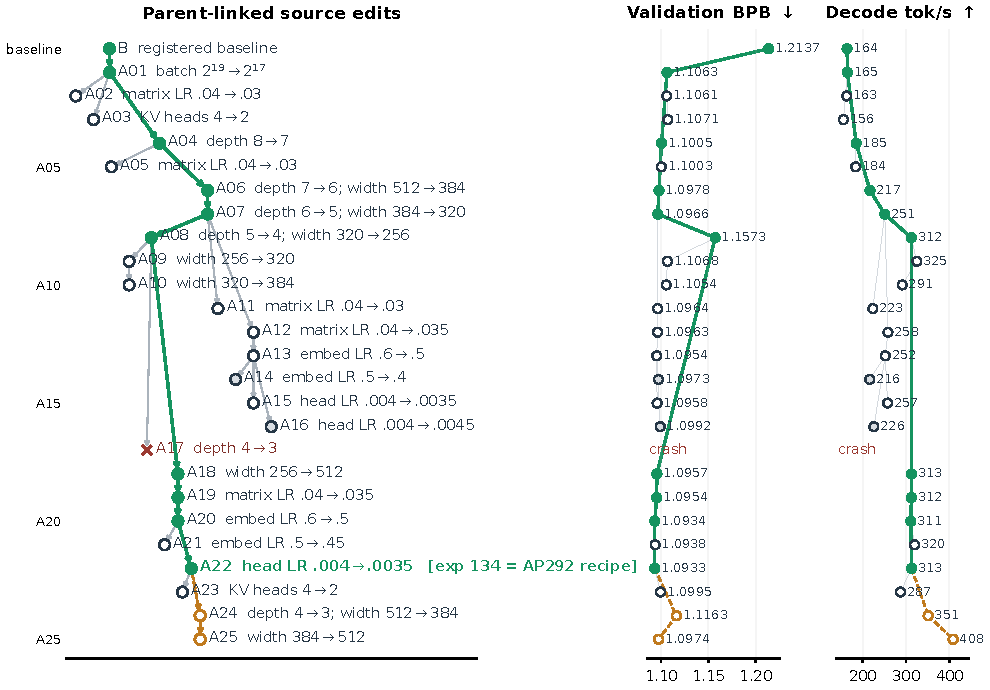
\includegraphics[width=\linewidth]{figures/autopareto_lineage.pdf}
\caption{The seed-0 autonomous discovery lineage. Every attempt is shown against its measured discovery objectives, with arrows encoding recorded parentage. The highlighted path ends at A22, global archive experiment 134, the frozen recipe later retrained as AP292. The dashed A24 to A25 branch pursues throughput and is not used for the headline. Open nodes are retained alternatives, gray nodes are dominated, and the crashed A17 attempt is preserved.}\label{fig:lineage}
\end{figure}

\paragraph{What the agent changed.} Across the 75 attempts of the three campaigns, a source-diff audit labels 32 edits as architectural, 21 as optimizer changes, 10 as optimization logic, eight as batching, and four as schedule changes. Figure~\ref{fig:lineage} shows the complete seed-0 campaign. The path to the selected recipe runs baseline $\rightarrow$ A1 $\rightarrow$ A4 $\rightarrow$ A6 $\rightarrow$ A7 $\rightarrow$ A8 $\rightarrow$ A18 $\rightarrow$ A19 $\rightarrow$ A20 $\rightarrow$ A22. It is not a monotonic descent. The aggressive compression at A8, which took the model to four layers and 256 width, raised validation BPB from 1.0966 to 1.1573 and was scored as a quality failure. Restoring width at A18 recovered it to 1.0957, and three successive learning-rate edits on the matrix, embedding, and output-head parameter groups reached 1.0933 at A22. A separate later branch, A24 to A25, traded quality for 408.4 tokens/s in the discovery workload. The interesting content of this trajectory is not that shallower models decode faster, which is expected, but that the recipe the contract selected emerged from an interaction between a failed compression and the optimizer edits that repaired it.

\paragraph{What the agent said it was doing.} Each attempt carries a hypothesis recorded before the patch was applied, which lets us read the search rather than only its outcome. The exposure incentive is visible in that text. Proposing the compression at A8, the agent predicted that "reducing depth from five to four under the unchanged aspect rule will preserve or improve validation BPB because the smaller model processes more tokens in the fixed training time, while further increasing cached decode speed and reducing inference memory." The rationale is explicitly two-part, and the second part is about the contract rather than the model. The prediction was wrong on quality, and the agent then reversed course: at A18 it proposed to change "only ASPECT\_RATIO from 64 to 128" so that "increasing depth-four width from 256 to 512 will recover enough validation quality to establish a new high-quality frontier point while retaining the cached-decode benefit of only four layers." The final three edits on the selected path are single-hyperparameter moves on that recovered architecture, ending at A22 with "reducing UNEMBEDDING\_LR from 0.004 to 0.0035 will improve or preserve validation BPB while potentially recovering cached-decode speed, with architecture memory unchanged." The agent therefore did not stumble onto a shallow-wide model; it compressed too far, measured the damage, restored width, and then tuned the three parameter-group learning rates one at a time.

\paragraph{Identifiers.} A22 is attempt 22 of the seed-0 campaign and is global archive experiment 134. AP292 denotes that attempt's frozen source recipe as retrained under the verification protocol; the numeral is inherited from archive row 292, an earlier exact-source confirmation of experiment 134 on seed 1, so AP292 names a configuration rather than a separately discovered architecture. AP299 and AP294 name the frozen recipes of A25 (experiment 137) and A24 (experiment 136).

\paragraph{Exposure was not held fixed.} Table~\ref{tab:main} lists what each recipe actually consumed under the 300-second contract. The spread is large: 88.9M tokens for the quality-only comparator against 251.8M for the fastest AutoPareto recipe. AP292 trained on 159.8M tokens, 1.80 times the comparator's exposure, and beat it on validation BPB by 0.0017. A margin that small, obtained with that much extra data, is not evidence about the programs alone.

\section{Matched-exposure verification}\label{sec:verify}
\paragraph{Design.} We froze seven recipes as exact source files and retrained each at seeds 3, 4, and 5 for exactly 201,326,592 counted tokens. That budget is $192\times2^{20}$ and is divisible by both batch settings present in the panel (1{,}536 updates of 131{,}072 tokens, or 384 updates of 524{,}288), so every recipe stops on an exact optimizer update with no partial step. The seeds are disjoint from every seed used during discovery (0, 1, 42) and from an earlier exact-source confirmation stage (0, 1, 2). The panel contains the registered baseline; the best completed attempt of the recovered quality-only AutoResearch archive, which is the strongest verification-compatible reference; the TPE and MOTPE quality representatives from the classical archives; and three AutoPareto recipes chosen before verification under the archive's primary selection roles for best quality, largest exclusive hypervolume contribution, and fastest within one percent of best quality. Selection is recorded in campaign identifiers created on 2026-08-10 and executed from 2026-08-12, so it preceded verification. Quality is scored as held-out BPB on a separate fixed shard prefix, distinct from the validation stream used during search.

\begin{table}[t]
\caption{Discovery-stage exposure and matched-exposure verification. The two discovery columns come from each recipe's originating archive attempt under the 300-second contract, where exposure varied by design. The remaining columns come from retraining the frozen recipe at exactly 201,326,592 counted tokens on seeds 3, 4, and 5, and are means over those three seeds; SD is the sample standard deviation of held-out BPB. Decode is cached-decode tokens/s, MiB is peak allocated inference memory, KV MiB is measured incremental KV-cache memory, and steady seconds is a sustained-rate training estimate from timed post-warm-up updates rather than end-to-end runtime. Memory and KV are deterministic for this workload and identical across all repetitions and seeds.}\label{tab:main}
\centering\small\begin{tabular}{lrrrrrrrrr}
\toprule
Recipe & M par. & Disc.\ Mtok & Disc.\ val BPB $\downarrow$ & Held-out BPB $\downarrow$ & SD & Decode $\uparrow$ & MiB $\downarrow$ & KV MiB $\downarrow$ & Steady s \\
\midrule
Baseline & 50.33 & 92.8 & 1.2127 & 1.1466 & 0.0047 & 196.8 & 250.9 & 3.984 & 689 \\
AutoResearch & 50.33 & 88.9 & 1.0950 & 1.0998 & 0.0019 & 192.9 & 250.9 & 3.984 & 696 \\
TPE & 39.85 & 113.8 & 1.0977 & 1.1194 & 0.0043 & 258.9 & 205.9 & 2.988 & 541 \\
MOTPE & 26.35 & 153.0 & 1.0981 & 1.1483 & 0.0031 & 270.0 & 145.6 & 2.241 & 398 \\
AP292 & 29.36 & 159.8 & 1.0933 & 1.1418 & 0.0060 & 383.0 & 162.9 & 1.992 & 385 \\
AP299 & 26.21 & 197.7 & 1.0974 & 1.1593 & 0.0004 & 488.3 & 142.4 & 1.494 & 313 \\
AP294 & 17.89 & 251.8 & 1.1163 & 1.1901 & 0.0022 & 495.5 & 106.9 & 1.121 & 296 \\
\bottomrule
\end{tabular}

\end{table}

\begin{figure}[t]
\centering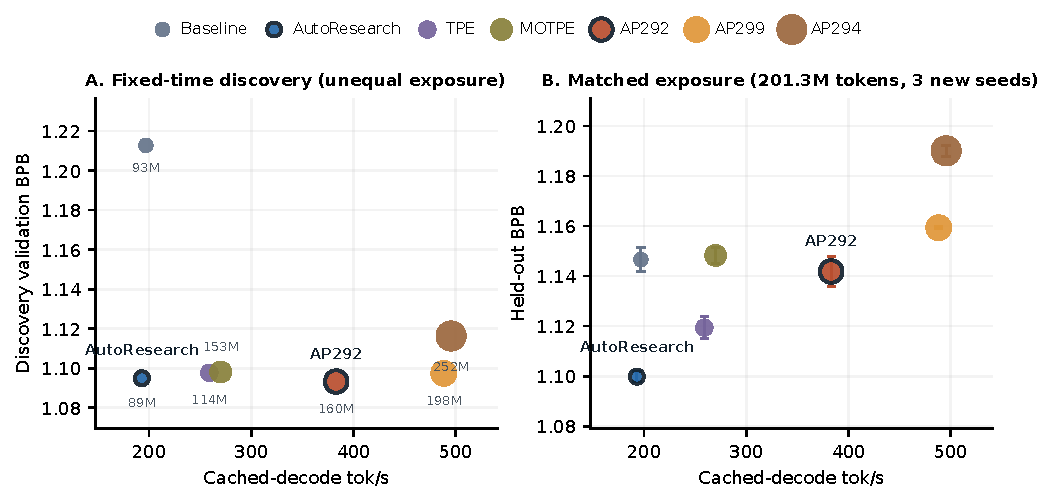
\includegraphics[width=\linewidth]{figures/discovery_vs_verification.pdf}
\caption{What the contract selected against what survived. Both panels place each frozen recipe at its verified cached-decode throughput, so only the quality axis changes between them. Panel A shows discovery-stage validation BPB from the fixed-time campaigns, with each marker sized and annotated by the training tokens that candidate actually received. Panel B shows held-out BPB after retraining every recipe at 201.3M tokens on three unseen seeds, with sample SD across seeds. The vertical ordering of AP292 and AutoResearch inverts between the panels, and the AP292 margin in panel A (0.0017 BPB) is far smaller than the AutoResearch margin in panel B (0.042 BPB).}\label{fig:dv}
\end{figure}

\paragraph{The ranking changes.} AP292 and the AutoResearch reference are unusually well matched for this comparison: both complete 1,536 optimizer updates at total batch size 131,072, so they agree on tokens, updates, and batch. Under matched exposure the quality ordering nonetheless inverts. AutoResearch reaches held-out BPB 1.0998 against 1.1418 for AP292, a gap of 0.042 in the opposite direction to the 0.0017 discovery-stage margin. The reordering is not confined to that pair: TPE moves from fourth to second, AP299 from third to sixth, and the untouched baseline from last to fourth. Figure~\ref{fig:dv} shows the two orderings side by side. We do not attribute the reversal to exposure alone, because verification also changed the seeds and the evaluation data; what the experiment establishes is that the fixed-time ranking did not survive an exposure-controlled retest, which is sufficient to disqualify it as a recipe-quality ranking.

\paragraph{The efficiency result survives.} Every deployment quantity in Table~\ref{tab:main} is measured on the verified checkpoints under one protocol. AP292 decodes at 383.0 tokens/s against 192.9 for AutoResearch, a factor of 1.99, with 29.36M against 50.33M parameters, 162.9 against 250.9 MiB of peak allocated inference memory, and 1.992 against 3.984 MiB of incremental KV-cache memory. The last of these is not merely proportional to depth but exactly predicted by it. With $L$ layers, $h_{kv}$ key-value heads of dimension $d$, two tensors per layer, two bytes per BF16 element, and 255 generated positions, the incremental cache is $255\cdot 2\cdot 2\cdot L\,h_{kv}d$ bytes. For AP292 that is $255\cdot2\cdot2\cdot4\cdot4\cdot128=2{,}088{,}960$ bytes, or 1.9922 MiB, which is the measured value to the last digit; the same expression reproduces the measured KV column for all seven recipes exactly. The measurement is therefore doing what we think it is doing. Peak memory and KV state are deterministic for this workload and identical across all 30 measured repetitions and all three seeds, so their variability is zero rather than merely small; only throughput varies, and its seed-level SD is 4.9 tokens/s against a 190 tokens/s difference. The cost is 0.042 held-out BPB. AP292 remains nondominated in the three-objective sense: no recipe in the panel is at least as good on held-out BPB, throughput, and memory simultaneously.

\section{Instrumentation: what had to be repaired}\label{sec:repairs}
The results above rest on two instruments, the training-budget boundary and the decode benchmark, and neither worked correctly at first. We report the failures because each changed a number a reader would otherwise take at face value.

\subsection{Enforcing the training budget}
A contract that is not enforced is not a contract, and the first failure here is an instance of exactly the leak this paper is about, one level lower in the stack.

\paragraph{Untimed warm-up was donating free training.} The original protected launcher performed the first eleven optimizer updates as ordinary training but excluded them from the timed interval, computing measured tokens as $(\text{step}-11)\times\texttt{TOTAL\_BATCH\_SIZE}$. Those eleven updates were real: gradients were applied and weights moved. At the baseline batch of 524,288 tokens per update, each candidate therefore received $11\times524{,}288=5{,}767{,}168$ tokens of learning outside its own budget, and the amount scaled with whatever batch size the agent chose. This is resource leakage of the same kind as the fixed-time exposure confound, one level lower in the stack: a candidate could increase its unbudgeted head start by editing a batch constant. The historical baseline records 92,798,976 tokens over 177 total updates, and a later calibration 93,847,552 over 179, both inclusive of that prefix.

\paragraph{The first repair traded one leak for another.} The obvious fix was to run warm-up in a separate process and destroy it, so that no gradient, optimizer moment, RNG state, dataloader position, or counter could survive into scientific training. That is correct as far as learned state goes, and it is what we did first. Destroying the process also destroyed the CUDA context, the TorchInductor compiled kernels, and allocator warmth, so the first scientific update in the fresh process paid lazy initialization inside the protected 300 seconds. Measured first-update times were 20.946 s, 20.809 s, and 25.674 s against a steady-state 1.782 to 1.784 s per update, and the recalibrated baseline exposure collapsed to 82,837,504, 82,837,504, and 81,264,640 tokens, that is 158, 158, and 155 updates.

\paragraph{Arithmetic, not instrumentation, caught it.} A baseline that had been recording 179 updates should record $179-11=168$ once the eleven-update prefix stops counting, which is $168\times524{,}288=88{,}080{,}384$ tokens. The measurement said 158 updates and 82.8M tokens. The 10-update, 5,242,880-token shortfall corresponds to $10\times1.783\approx17.8$ s, which sits inside the 20.8 to 25.7 s that the first update was observed to take. The deficit was therefore accounted for by initialization charged to the scientific budget, not by any change to training mathematics, and the correct response was to move that initialization out of the budget rather than to accept a smaller one.

\paragraph{The final lifecycle.} One worker process is kept alive throughout. A disposable warm-up model absorbs compilation and CUDA kernel initialization, is discarded, and the scientific model, optimizer, CPU and CUDA RNG, dataloader position, and counters are reconstructed from the registered source and seed. The controller then asserts that the reconstructed initial-state hash equals the hash taken before warm-up, \texttt{b2db8781}, so the process retains its compiled and allocator warmth while carrying zero learned state across the boundary. The first scientific update after the repair takes 1.711 s against a steady 1.783 s, that is, it is already steady-state. Recalibrating the baseline under this lifecycle gave 88,604,672, 88,080,384, and 88,604,672 tokens, whose median under the registered rule $N^{*}=\lfloor \text{median}/524288\rfloor\times524288$ fixes the fixed-token contract at 88,604,672 tokens, or exactly 169 updates. The predicted 168 and the measured 169 differ by one update, which is the resolution of the instrument.

The three calibration values are kept distinguishable in the record rather than overwritten: 93,847,552 as superseded historical, 82,837,504 as a cold-start artifact explicitly marked unusable for any study attempt, and 88,604,672 as the registered budget. The contract in this paper is therefore 300.000 seconds of \emph{scientific} training, with initialization outside it and no learned state entering it.

\subsection{Measuring cached decoding}\label{sec:inference}
The throughput and memory numbers carry the deployment claim, so the instrument that produces them needs its own argument. Two properties matter: the cached path must be correct, and the timing must be attributable to the model rather than to the backend.

\paragraph{Correctness must be checked before speed.} A candidate that may rewrite \texttt{train.py} can define its own attention, and a broken key-value cache is fast for the wrong reason. Before any timing, the protected evaluator runs a teacher-forced comparison over 32 decode steps: at each step it computes a full-prefix reference over the common prefix with no prior cache state, computes the corresponding one-token cached step, and requires exact greedy-token agreement plus a bound on the logit difference.

\paragraph{The reference has to be SDPA, not the candidate's own forward.} The candidate's \texttt{forward} may dispatch a hardware-specific kernel, in our case FlashAttention-3, while the protected cache uses scaled dot-product attention. Comparing those two measures the round-off difference between two attention backends, not whether the cache is correct. The evaluator therefore uses its own SDPA full-prefix pass as the reference and recomputes it on each common prefix, so that the only cached-state code under test is \texttt{decode\_one}.

\paragraph{Why BF16 alone cannot adjudicate, and why we did not move the threshold.} The screening bound is a mean absolute logit error of 0.03 in BF16. BF16 carries an eight-bit mantissa, a relative resolution near $3.9\times10^{-3}$; over 2,048-position attention sums and several residual blocks, two orderings of the same arithmetic on logits of order ten disagree at the level of hundredths without either being wrong. That is what the AutoResearch reference did: greedy tokens agreed at all 32 steps, but the maximum mean absolute logit error was 0.04805, peaking at a single-coordinate error of 0.15288 at step 14, so it failed a 0.03 screen it had no business failing on cache semantics. The candidate's own BF16 FlashAttention forward against the cached SDPA path disagreed similarly, at 0.04034. Raising the threshold would have been the easy repair and the wrong one, because it would have widened the gate for real cache bugs at the same time. We left 0.03 unchanged and added an adjudicator instead.

\paragraph{FP32 adjudication.} When greedy tokens all agree but the BF16 screen fails, the same comparison is rerun in float32 against tighter bounds, mean error at most $10^{-5}$ and maximum error at most $10^{-4}$. Float32 has a 24-bit mantissa, so summation-order effects fall roughly four orders of magnitude below the BF16 level and any residual disagreement is attributable to the cache rather than to arithmetic. The AutoResearch case adjudicated at a maximum mean error of $2.18\times10^{-6}$, four orders inside the bound, which settles it: the cache is exact and BF16 round-off produced the screen failure. Official throughput and memory remain BF16 with FlashAttention; float32 is a referee, never a reported measurement.

Building that referee produced its own bug worth recording. The first adjudication host converted the whole model to float32 and called the candidate forward, which routed float32 queries, keys, and values into FlashAttention and raised \texttt{FlashAttention only supports fp16, bf16, and fp8\_e4m3 data type}. The kernel is correct to refuse; the integration was wrong. The fix keeps FlashAttention for official BF16 inference and routes float32 adjudication through protected SDPA, which supports it, leaving the measured quantities untouched.

\paragraph{Timing and its residual risk.} Each verification run performs adaptive stabilization generations followed by 30 measured repetitions in three passes, with per-pass coefficient-of-variation and median-drift gates, and records CUDA-event timing alongside synchronized host timing as a cross-check. The reported figure is the per-run median over the 30 repetitions and then the mean over seeds; the seed-level SD for AP292 is 4.9 tokens/s. We do not claim the instrument is universally reliable. In six fresh diagnostic sessions on the current paired study, five were rejected before producing a usable scalar and the sixth failed its final drift gate, with GPU telemetry showing no thermal or power throttling and no competing process, which points at low-utilization decode scheduling variance. That is why the paired study in Section~\ref{sec:contract} promotes no throughput value, and why the deployment claims in this paper rest only on the verification panel, where all 21 runs passed the stability gates.

\section{Downstream evaluation}\label{sec:downstream}
The frozen evaluation suite was fixed before verification and was never visible to the agent. It scores zero-shot likelihood on ARC-Easy test (2,376 items), PIQA validation (1,838), LAMBADA test (5,153), and BLiMP (67,000 minimal pairs across 67 configurations), in raw and length-normalized form where both are defined. Because the 67 BLiMP configurations contain exactly 1,000 pairs each, macro and micro accuracy coincide, and we report one column.

\begin{table}[t]
\caption{Complete frozen downstream suite after matched-exposure retraining. Entries are mean $\pm$ sample standard deviation over seeds 3, 4, and 5. Accuracies are percentages and LAMBADA perplexity is lower-is-better; held-out BPB for the same runs is in Table~\ref{tab:main}. Most between-recipe differences are comparable to or smaller than the seed-level variation, and we make no significance claim.}\label{tab:downstream}
\centering\footnotesize\setlength{\tabcolsep}{4pt}\begin{tabular}{lrrrrrrr}
\toprule
Recipe & ARC-E $\uparrow$ & ARC-E$_n$ $\uparrow$ & PIQA $\uparrow$ & PIQA$_n$ $\uparrow$ & LMB acc $\uparrow$ & LMB PPL $\downarrow$ & BLiMP $\uparrow$ \\
\midrule
Baseline & 35.28\,\tiny$\pm$1.48 & 33.33\,\tiny$\pm$0.26 & 57.36\,\tiny$\pm$0.42 & 57.69\,\tiny$\pm$0.27 & 20.47\,\tiny$\pm$0.61 & 14.35\,\tiny$\pm$0.57 & 71.37\,\tiny$\pm$0.82 \\
AutoResearch & 36.50\,\tiny$\pm$1.37 & 32.44\,\tiny$\pm$0.93 & 58.67\,\tiny$\pm$1.37 & 57.25\,\tiny$\pm$1.43 & 20.44\,\tiny$\pm$0.93 & 14.15\,\tiny$\pm$1.00 & 74.56\,\tiny$\pm$0.59 \\
TPE & 35.70\,\tiny$\pm$1.01 & 32.46\,\tiny$\pm$1.22 & 57.64\,\tiny$\pm$0.71 & 56.08\,\tiny$\pm$0.90 & 21.42\,\tiny$\pm$1.26 & 13.92\,\tiny$\pm$1.45 & 73.30\,\tiny$\pm$0.78 \\
MOTPE & 35.41\,\tiny$\pm$1.81 & 33.96\,\tiny$\pm$1.57 & 57.45\,\tiny$\pm$0.45 & 56.57\,\tiny$\pm$0.33 & 21.53\,\tiny$\pm$2.27 & 15.06\,\tiny$\pm$1.73 & 72.47\,\tiny$\pm$0.55 \\
AP292 & 36.91\,\tiny$\pm$0.36 & 34.16\,\tiny$\pm$1.29 & 58.29\,\tiny$\pm$0.26 & 57.91\,\tiny$\pm$0.42 & 21.50\,\tiny$\pm$1.85 & 14.21\,\tiny$\pm$1.63 & 72.02\,\tiny$\pm$0.36 \\
AP299 & 35.68\,\tiny$\pm$1.56 & 32.56\,\tiny$\pm$1.94 & 57.27\,\tiny$\pm$0.74 & 56.33\,\tiny$\pm$1.36 & 20.76\,\tiny$\pm$0.21 & 15.60\,\tiny$\pm$0.73 & 70.47\,\tiny$\pm$0.71 \\
AP294 & 34.83\,\tiny$\pm$0.88 & 33.05\,\tiny$\pm$0.90 & 56.91\,\tiny$\pm$0.24 & 56.27\,\tiny$\pm$0.30 & 19.92\,\tiny$\pm$0.61 & 17.71\,\tiny$\pm$0.48 & 69.33\,\tiny$\pm$1.05 \\
\bottomrule
\end{tabular}

\end{table}

Table~\ref{tab:downstream} gives the complete suite for all seven verified recipes. Two patterns are worth separating. First, on the four task-accuracy metrics AP292 is at or near the top of the panel despite having 41.7\% fewer parameters than the AutoResearch reference: it has the best ARC-Easy accuracy (36.91) and the best length-normalized ARC-Easy (34.16) and PIQA (57.91) scores, and its LAMBADA accuracy of 21.50 is within 0.03 of the panel best. It trails AutoResearch on raw PIQA accuracy by 0.38 and on LAMBADA perplexity by 0.06. These are small differences set against seed-level standard deviations that reach 1.4 to 2.3 points on several of these metrics, so the honest reading is that AP292 and AutoResearch are not separated by these tasks at $n=3$. The defensible statement is the conditional one: halving depth cost nothing measurable on these four metrics at this scale.

Second, BLiMP does separate them, in the direction held-out BPB predicts: 72.02 for AP292 against 74.56 for AutoResearch, with seed SDs of 0.36 and 0.59. AP292 is lower on 51 of the 67 configurations, tied on 1, and higher on 15, and the deficits are not spread uniformly. They concentrate in negative-polarity-item scope and licensing, quantifier scope, filler-gap dependencies, agreement across an intervening distractor, and ellipsis.

\paragraph{Why those phenomena and not the others.} The two recipes are closer architecturally than the parameter counts suggest, which narrows the candidate explanations. Both are 512 wide with four query and four key-value heads at head dimension 128. They differ in depth, 4 blocks against 8, and in window pattern: AP292 uses \texttt{SSSL}, three half-context layers followed by one full-context layer, while the AutoResearch reference uses \texttt{SSSS}, eight half-context layers and no full-context layer at all. Receptive field is therefore not the explanation, and in fact runs the wrong way: AP292 devotes a quarter of its layers to full-context attention and the reference devotes none. BLiMP minimal pairs are also short, comfortably inside the half-context window, so neither model is truncating the evidence it needs.

What differs is sequential composition budget. Each residual block affords one round of attention-mediated movement of information between positions followed by one position-wise nonlinearity, so the number of blocks bounds how many dependent relational steps the model can chain before it must emit a logit. The phenomena where AP292 loses ground are the ones that require at least two such steps: resolving which noun phrase is the structural subject when a closer distractor noun disagrees in number, and only then propagating that resolved feature to the verb; locating a licensor and then evaluating an item within its scope; binding a filler to a gap site and then scoring the position that the gap makes available. Phenomena that reduce to a local selectional or lexical preference need fewer steps and are where the two models agree. ARC-Easy and PIQA, scored as likelihood over short continuations, lean mostly on lexical and world-knowledge association, which lives in the embeddings, the unembedding, and the width-512 position-wise MLPs. AP292 kept that width. Its lineage in Figure~\ref{fig:lineage} is precisely a model that gave up depth (8 to 4) and then bought width back (256 to 512 at A18), which is the configuration that would preserve associative capacity while spending composition depth.

We flag this as a mechanistic reading consistent with the measurements rather than an established cause. The supporting evidence is indirect: across the seven verified recipes BLiMP tracks held-out BPB at $r=-0.969$ and depth at $r=0.717$, and depth and held-out BPB are themselves entangled in this panel, so the correlation cannot separate them. A controlled ablation that varies depth at fixed width, fixed parameter count, and fixed token exposure would test the claim directly, and we have not run it.

Taken together, the efficiency gains of AP292 do not come with a broad collapse in downstream capability. They come with a measurable likelihood cost that surfaces on the metric with the least sampling noise and, within that metric, on the phenomena that need the most composition. The two more aggressive AutoPareto recipes make the trade explicit: AP299 and AP294 are faster and smaller than AP292 and worse on held-out BPB and on nearly every downstream metric, which is what a frontier should look like.

\section{Resource contracts as an experimental variable}\label{sec:contract}
Section~\ref{sec:verify} shows that a fixed-time contract can produce a quality ranking that does not survive controlled retraining. A separate question is whether the contract also changes what the agent chooses to try. We registered a prospective paired study to test this: two arms with identical staged code, identical agent configuration, and identical training seed, differing only in the stopping rule and the schedule-progress variable. Arm T trains for 300.000 protected seconds and completes the final update. Arm N processes exactly 88,604,672 counted tokens, the largest multiple of the 524,288-token quantum not exceeding the median token count of three seed-3 baseline runs under contract T. Learning-rate progress follows elapsed-time fraction in T and counted-token fraction in N. The registered hypothesis is nondirectional. Table~\ref{tab:controls} lists the executed controls.

\begin{table}[t]
\caption{Executed controls for the paired budget study. The staged code, agent configuration, and training seed are shared; the stopping rule and the schedule-progress variable differ by design. Provider-side agent state is not observable.}\label{tab:controls}
\centering\small\begin{tabular}{p{1.2in}p{1.8in}p{1.8in}}
\toprule
Control & Fixed time (T) & Fixed tokens (N) \\
\midrule
Initial code / loader & Identical executed input bytes & Identical executed input bytes \\
Scientist / seed & gpt-5.6-sol, high / 3 & gpt-5.6-sol, high / 3 \\
Training stop & 300 s; complete final update & 88,604,672 counted tokens \\
LR progress & Elapsed-time fraction & Counted-token fraction \\
Frozen prefix & 4 completed attempts & 4 completed attempts \\
Inference / memory & Shared bracketed protocol & Shared bracketed protocol \\
Context / hardware & Separate history; one A40 & Separate history; same A40 \\
Parent policy (executed) & Quality-valid parents allowed & Quality-valid parents allowed \\
\bottomrule
\end{tabular}

\end{table}

\begin{table}[t]
\caption{Completed attempts in the paired budget study at the analysis freeze: four per arm. Each arm is a single adaptive trajectory in which every attempt may depend on its predecessors, so these are not eight independent samples and support no causal estimate.}\label{tab:budget}
\centering\small\begin{tabular}{lrrrrr}
\toprule
Trial & Depth & M params & M tokens & Updates & BPB \\
\midrule
T1 & 8 & 50.33 & 87.818 & 335 & 1.1748 \\
T2 & 8 & 50.33 & 86.639 & 661 & 1.1034 \\
T3 & 8 & 50.33 & 82.838 & 1264 & 3.2159 \\
T4 & 8 & 50.33 & 82.838 & 1264 & 3.2159 \\
N1 & 10 & 85.85 & 88.605 & 169 & 1.1631 \\
N2 & 12 & 135.27 & 88.605 & 169 & 1.1643 \\
N3 & 10 & 85.85 & 88.605 & 338 & 1.1243 \\
N4 & 10 & 85.85 & 88.605 & 676 & 1.1402 \\
\bottomrule
\end{tabular}

\end{table}

Table~\ref{tab:budget} reports the completed prefix, four attempts in each arm. We describe it and draw no causal conclusion. In the fixed-token arm the first two edits add capacity, taking the model from 50.33M to 85.85M and then 135.27M parameters, with validation BPB moving from 1.1631 to 1.1643; the third attempt returns to the first arm parent and halves the batch, reaching 1.1243 at 338 updates, and the fourth halves it again to 676 updates and 1.1402. In the fixed-time arm the architecture stays at 50.33M parameters throughout and the edits change batching and learning rate, reaching 1.1034 at 661 updates, after which two attempts complete with validation BPB near 3.216 following a learning-rate rescale. No attempt in either arm is yet Pareto-eligible under the deployment criteria, so the prefix supports no frontier claim. What it does establish is that the instrument runs end to end under both contracts with matched inputs, which is the prerequisite for the replicated study described in Section~\ref{sec:limits}.

\section{Auditability and reproducibility}\label{sec:repro}
The claim that an autonomous system discovered something is only as good as the record of what it did. Every attempt in this project retains the agent's stated hypothesis and intended change, the applied patch, the parent identifier, the source SHA-256, the parent hash, the run status, the raw metrics, the checkpoint hash, and the campaign view that was returned to the next call. Crashes, corrupt registrations, protocol incompatibilities, and technically complete but scientifically poor runs remain in the record with their failure text rather than being filtered out.

The analysis pipeline that produced every number in this paper is separate from the pipeline that produced the experiments, and it launches nothing. It re-derives results from frozen artifacts: raw training metrics, checkpoints, inference records, downstream databases, agent prompts, manifests, and candidate sources. For each of the 21 verification runs it checks the recipe source hash against both the training record and the public manifest, the exact 201,326,592-token total, the update count against tokens per update, one timing row per optimizer update, the checkpoint-to-downstream pairing, the completeness of the nine-metric suite, and the evidence cutoff. It also checks metric direction, so that a lower-is-better quantity cannot be silently inverted. Every table and vector figure in this paper is regenerated by that pipeline.

Table~\ref{tab:repro} states what is preserved and what is publicly available, which are not the same thing. The distinction matters: a reader can re-derive every reported number from the released aggregate records and frozen recipe sources, but cannot currently re-run training from released checkpoints, because checkpoints and raw logs are retained privately rather than published.

\begin{table}[t]
\caption{Artifact status. Preserved means the artifact exists in the project record and was used by the audit; released means it is in the public artifact set.}\label{tab:repro}
\centering\small
\begin{tabular}{lll}
\toprule
Artifact & Status & Detail \\
\midrule
Frozen recipe sources & Preserved, released & Seven exact \texttt{train.py} files with SHA-256 \\
Protocol manifests & Preserved, released & Token budget, seeds, batch settings, hardware \\
Aggregate result summaries & Preserved, released & Per-seed training, inference, and downstream values \\
Agent hypotheses and patches & Preserved & Per attempt, including failures \\
Parent lineage and hashes & Preserved & Parent identifier plus source and parent SHA-256 \\
Registered contracts and prompts & Preserved & Program text, staged context, executed instruction diff \\
Raw inference repetitions & Preserved & 30 measured repetitions per verification run \\
Downstream raw outputs & Preserved & Nine metrics per run, per seed \\
Failure records & Preserved & Crashes, corrupt rows, uncertain timing \\
Model checkpoints & Preserved, not released & Retained privately; not in the public artifact set \\
Raw training logs and telemetry & Preserved, not released & Retained privately \\
\bottomrule
\end{tabular}
\end{table}

\paragraph{Human and agent attribution.} The agent proposed every source patch in the campaigns, together with the hypothesis recorded before each patch. The harness executed training and all measurement. Humans specified the three objectives, the 300-second contract, the editable surface, the matched-exposure verification design, the seven frozen recipes, the comparator, and the interpretation reported here. Humans also did the debugging described in Sections~\ref{sec:repairs} and~\ref{sec:inference}: finding the untimed warm-up leak, diagnosing the cold-start regression by arithmetic, designing the same-worker lifecycle with hash-verified state reconstruction, deciding to adjudicate the correctness screen in float32 rather than loosen it, and routing that adjudication through SDPA once FlashAttention refused float32 inputs. Humans also amended parent eligibility to admit quality-valid but speed-uncertain candidates and relaunched campaigns. One deviation is disclosed rather than smoothed over: the registered program text specifies that the eleven disposable warm-up updates run in a separate process, whereas the executed controller runs them in the same worker, discards that model, reconstructs scientific state, and verifies matching initial-state hashes before measurement. That deviation is the deliberate outcome of the second repair, not an oversight, and the reason for it is the cold-start cost documented above. Where preserved artifacts do not identify whether an intervention originated with the human operator or with assisted debugging, we exclude it from claims of autonomous contribution rather than guessing.

\section{Related work}
Architecture search for efficient Transformers is well established. Primer searches compositions of low-level operations and recovers squared ReLU and depthwise convolutions around attention projections \citep{primer}, a stronger form of operator-level novelty than the numerical architecture edits our agent made; squared ReLU was already present in our baseline, so AutoPareto did not discover it. einspace searches a grammar of primitive operations \citep{einspace} and MOTE-NAS combines landscape and convergence estimates for multi-objective search \citep{mote}. MONAQ queries a language model for multi-objective architectures targeted at constrained devices \citep{monaq}, so neither multi-objective search nor language-model-driven architecture generation is new here.

A second line studies agents that conduct research rather than only search architectures. AutoDiscovery, MLE-STAR, AI-Researcher, and MLE-Dojo address open-ended hypothesis search, targeted refinement, broader research automation, and interactive ML engineering environments \citep{autodiscovery,mlestar,airesearcher,mledojo}. Ferreira et al.\ evaluate language-model-driven optimization against classical hyperparameter optimization in the autoresearch setting and find that classical methods remain strong baselines \citep{ferreira}, consistent with our own archives, in which the fixed-vector optimizers land within 0.005 validation BPB of the coding agents. Classical resource allocation across configurations, as in Hyperband and BOHB \citep{hyperband,bohb}, is the closest existing treatment of budget as a first-class object, but it allocates within a fixed configuration space and does not face the case where the searched program changes its own throughput.

The gap sits between these lines: efficient-architecture search largely assumes a fixed training protocol, and autonomous-research systems are usually reported through the score their contract produced. We combine an auditable autonomous source-edit trajectory, a resource-sensitive search contract, and post-search matched-exposure verification, and show that the third changes the conclusion the first two would otherwise support. We are not aware of prior work that verifies an autonomous architecture discovery under an exposure-controlled retest.

\section{Discussion, limitations, and broader impact}\label{sec:limits}
\paragraph{What the result does and does not license.} The efficiency finding is a direct measurement on verified checkpoints under one protocol, and we state it without hedging. The quality finding is a negative result about an ordering, and because verification changed exposure, seeds, and evaluation data together it does not isolate exposure as the cause. Nor does it isolate architecture: AP292 is a complete recipe whose architectural, optimizer, batching, and schedule changes remain bundled.

\paragraph{Scope.} All results are from one GPU family, one model family below 51M parameters, one dataset, and one cached-decoding workload at batch one with short context. We make no scale-transfer, cross-GPU, or energy claim, and the artifacts contain no energy accounting that would support one. Three verification seeds estimate recipe variability, not search-policy variability. The classical archives differ from the coding agents in search space, budget, seed, and failure history, so Table~\ref{tab:main} places them alongside the agents for context and not as a controlled tournament, and the paired budget study is one incomplete adaptive trajectory per arm. Finally, the agent is a proprietary service whose internal state we cannot record, so exact reproduction of the search is unavailable even though every input, output, and artifact of the harness is preserved.

\paragraph{The experiment this paper motivates.} The continuation is a replicated contract study rather than a longer single trajectory: independent campaigns per contract, so that between-campaign variance can be estimated and the arm effect separated from trajectory noise, with edit categories, capacity, exposure, and achieved frontier pre-declared.

\paragraph{Broader impact.} The practical recommendation is narrow: publish the resource contract, including the stopping rule, the schedule-progress variable, the warm-up boundary, the inference workload, and the feedback returned after each attempt, because each determines what the agent is rewarded for finding. Section~\ref{sec:repairs} is the argument for the warm-up boundary in particular: a leak invisible to every score changed baseline exposure by six percent. Trajectories should retain crashes, unstable measurements, and poor-but-complete runs, and parent-eligibility rules should be recorded, since permitting a speed-uncertain candidate to seed later work changes the search policy. Efficiency results such as ours reduce the cost of one experiment without necessarily reducing total consumption, and small-model benchmarks establish nothing about safe use in consequential settings. As experiment volume grows the accountable object is the record, which should keep the human question, the agent's prediction, the edit, the outcome, and the retrospective explanation distinguishable.

\section{Conclusion}
An autonomous researcher optimizes what its contract measures. Under a fixed-time contract that lets the agent change training throughput, that measurement quietly includes how much data each candidate received, which here varied by a factor of 2.8 across the compared recipes. Retraining seven frozen recipes at matched exposure on unseen seeds removed the selected recipe's apparent quality advantage and left its deployment advantage intact, and enforcing the contract honestly first took three repairs, one of which had been handing every candidate 5.77M tokens of unbudgeted training. The autonomous search produced a genuine result; determining which result it was meant verifying it under a contract different from the one that found it.

\appendix
\section{Measurement protocol}\label{app:measure}
\paragraph{Inference and memory.} Protocol \texttt{autopareto\_inference\_stabilized\_v2}; the correctness and stability design is described in Section~\ref{sec:inference}. Workload: BF16, batch one, a fixed protected prompt of 256 input tokens, 256 generated tokens, greedy decoding, of which the 255 single-token cached steps after prefill are timed. Peak memory is \texttt{torch.cuda.max\_memory\_allocated()} after \texttt{reset\_peak\_memory\_stats()} at the start of each measured repetition, with the checkpoint already resident, so model weights are included and CUDA reserved memory is excluded; the window covers prefill and every measured decode step. Incremental KV memory is the validated cache size after the final decode step minus the size after prefill. Both memory quantities were identical across all 30 repetitions and all three seeds for every recipe in the panel.

\paragraph{Training.} Counted tokens exclude the eleven disposable warm-up updates. AP292, AP299, AP294, AutoResearch, TPE, and MOTPE use total batch 131,072 with device batch 64 and no gradient accumulation, giving 1,536 optimizer updates; the baseline uses total batch 524,288 with accumulation 4, giving 384 updates. Learning-rate progress is the fraction of the token budget consumed. Precision is BF16 on one NVIDIA A40 (driver 570.211.01) under PyTorch 2.9.1+cu128 with CUDA 12.8 and Python 3.12.

\paragraph{Data and recipe identity.} Training and validation use \texttt{karpathy/climbmix-400b-shuffle} at dataset revision \texttt{915333b4f8b8684f39aeaafea600fea6f43fb703} with 2,048-token packed sequences and a hashed project tokenizer of 8,192 entries. Held-out BPB is evaluated on shard \texttt{shard\_06541.parquet} over 2,560 segments and 5,242,880 tokens. Each recipe is identified by the SHA-256 of its exact \texttt{train.py}: baseline \texttt{428e22f1}, AutoResearch \texttt{b3a961ee}, TPE \texttt{8547b278}, MOTPE \texttt{62882a20}, AP292 \texttt{55a7fd8b}, AP299 \texttt{36e3ad91}, AP294 \texttt{6d0d8d1d}, with full digests in the released manifest and in every per-run training record.

\section{Disclosure}
This manuscript, its analysis code, and its figures were prepared with AI assistance. The research agent that produced the searched source edits is \texttt{gpt-5.6-sol} run through Codex CLI 0.153.0; the writing and analysis assistant is a separate general-purpose assistant. Records identify research-agent actions separately from human actions, and interventions whose authorship cannot be reconstructed from artifacts are excluded from claims of autonomous contribution. Authorship of this submission is human-only.

\clearpage
\bibliographystyle{plainnat}
\bibliography{references}
\end{document}
